\documentclass[]{article}
\title{ECO325: Lecture Notes \\ \small Advanced Economic Theory: Macro}
\author{Tianyu Du}
\date{\today}

\usepackage{spikey}
\usepackage{amsmath}
\usepackage{amssymb}
\usepackage{soul}
\usepackage{float}
\usepackage{graphicx}
\usepackage{hyperref}
\usepackage{xcolor}
\usepackage{chngcntr}

\counterwithin*{equation}{section}


\usepackage[
    type={CC},
    modifier={by-nc},
    version={4.0},
]{doclicense}


\begin{document}
    \maketitle
    \doclicenseThis
    \section*{Notes}
    	\paragraph{Github} \url{https://github.com/TianyuDu/Spikey_UofT_Notes}
    	\paragraph{Color notations}
    		\begin{itemize}
    			\item \textcolor{orange}{Important equations for model setup.}
    			\item \textcolor{blue}{Important equations as results from model.}
    			\item \textcolor{violet}{Implications of model result.}
    		\end{itemize}
    \paragraph{Revisions}
    \begin{itemize}
    	\item Revise October 2. 2018. Midterm 1.
    \end{itemize}
    \tableofcontents
    \newpage
    
    \section{Lecture 1. September 6. 2018}
        \begin{definition}
            A \textbf{growth miracle} are episodes where thee growth in a country far exceeds the world average over a extended period of time. \ul{Result} the country experiencing the miracle moves up the wold income distribution.
        \end{definition}
        
        \begin{definition}
            A \textbf{growth disaster} is an episodes where the growth in a country falls short at the world average for an extended period of time. \ul{Result} the country moves down in the world income distribution.
        \end{definition}
    
        \paragraph{Facts}(with corresponding result from Solow growth model.)
        \begin{enumerate}
            \item Real output($Y$) grows at a (more or less) constant rate ($n+g$).
            \item Stock of real capital($K$) grows at a (more or less) constant rate($n+g$) (but it grows faster than labor input($L$)($n$).
            \item Growth rates of real output and the stock of capital are about the same. (both $n+g$)
            \item The rate of growth of output per capita($\frac{Y}{L}$) varies greatly across countries. ($g$ varies across countries)
        \end{enumerate}
        
        \subsection{Solow Growth Model (continuous time version)}
            \paragraph{Intro.} Solow growth model decomposes the growth in output per capita into portions accounted for by increase in \ul{inputs} and the portion contributed to increases in \ul{productivity}.
           
            \paragraph{Notations} In the baseline model we denote $K$ as capital, $L$ as labor and $A$ as technology.
            
        \subsubsection{Production Function}
            \begin{remark}
                \st{Harrod-neutral technology here, refer to Uzawa's theorem.}
            \end{remark}
            \begin{definition}
                The \textbf{effective labor input}(total units off effective labor) is defined as $A(t)L(t)$
            \end{definition}
            
            \begin{definition}
                The production function is defined as a real-valued mapping from input factor space to an output level.
	            \begin{equation}
                    \textcolor{orange}{Y(t) = F(K(t), A(t)L(t))}
	            \end{equation}
            \end{definition}
            
            \begin{example}
            	    Cobb-Douglas form of production function.
                \[
                    Y(t) = K(t)^\alpha (A(t)L(t))^{1 - \alpha},\ \alpha \in (0, 1)
                \]
            \end{example}
            
            \begin{assumption} The production function is assumed to be \ul{constant return to scale} in $K$ and $AL$.
            \[
            	Y(cK, cAL) = cY(K, AL),\ \forall c \geq 0
            \]
           	This CRS assumption is the result of two separate assumptions.
           	\begin{enumerate}
           		\item \emph{The economy is big enough that the gains from specialization have been exhausted.} $\implies$ There is \textbf{no} increasing return to scale.
           		\item \emph{Inputs other than capital, labor, and the effectiveness of labor are relatively unimportant.} $\implies$ There is \textbf{no} decreasing return to scale.
           	\end{enumerate}
            \end{assumption}
            
            \begin{definition}
                Define $c := \frac{1}{AL}$, the \textbf{intensive form} of production function is
                \[
                    y(t) = \frac{Y(t)}{A(t)L(t)} = f(k(t))
                \]
                where $y := \frac{Y}{AL}$ denotes the \textbf{output per unit of effective labor} and $k := \frac{K}{AL}$ denote the capital stock per unit of effective labor.
            \end{definition}
	
	\section{Lecture 2 September 13. 2018}
		\subsection{Solow Growth Model: Setup}
			\begin{definition}
				\textbf{Production function} $F: \R^2_{+} \rightarrow \R_+$ maps input factors:
				\begin{itemize}
					\item $K(t) := $ aggregate capital stock at time $t$.
					\item $L(t) := $ aggregate labor supple at time $t$.
					\item $A(t) := $ labor argument technology\footnote{Harrod-neutral technology} (\ul{effectiveness of labor}) at time $t$.
				\end{itemize} 
				to output values ($Y(t) := $ aggregate output at time $t$.) The production function takes the form of
				\[
					Y(t) = F(K(t), A(t)L(t))
				\]
			\end{definition}
			
			\begin{assumption}[Assumptions on Production Function]
				The production function are assumed to be \ul{constant return to scale} in $A(t)L(t)$ and $K(t)$.
				\[
					cF(K(t), A(t)L(t)) = F(cK(t), cA(t)L(t)),\ \forall c > 0
				\]
			\end{assumption}
			
			\begin{definition}
				The \textbf{intensive form of production function} is defined as the output per unit of effective labor. \\
				Let 
				\[
					f(t) := \frac{Y(t)}{A(t)L(t)}
				\] 
				and 
				\[
					k(t) := \frac{K(t)}{A(t)L(t)}
				\] denote the output and capital per unit of effective labor respectively. By the assumption of \emph{CRS} on \emph{aggregate} production function, take $c = \frac{1}{A(t)L(t)}$. The \emph{intensive form} production function can be expressed as
				\begin{equation}
					\textcolor{orange}{
						y(t) = f(k(t))
					}
				\end{equation}
			\end{definition}
			
			\begin{assumption}[Assumptions on Intensive Form Production Function] the function $f(\cdot): \R_+ \rightarrow \R_+$ is assumed to satisfy \emph{Inada Conditions}.
				\begin{enumerate}
					\item $f(0) = 0$: capital is necessary for production.
					\item $f'(k) > 0,\ \forall k \in \R_+$: the marginal return of capital per effective unit of labor is positive.
					\item $f''(k) < 0,\ \forall k \in \R_+$: capital per effective unit of labor is experiencing diminishing marginal return.
					\item $\lim_{k \to 0}f'(k) = \infty$
					\item $\lim_{k \to \infty}f''(k) = 0$
				\end{enumerate}
			\end{assumption}
			
			\begin{remark}	
			The role of assumption 2.2 is to ensure that the path of the economy does not diverge.
			\end{remark}
			
			\begin{example}[Cobb-Douglas Production Function]
				Consider the Cobb-Douglas production function
				\[
					Y(t) = K(t)^\alpha (A(t)L(t))^{1 - \alpha},\ \alpha \in (0, 1)
				\]
				
				\begin{proof}[Check]
					Let $c \in \R_+$, 
					\begin{gather*}
						F(cK, cAL) = (cK)^\alpha (cAL)^{1 - \alpha} \\
						= c^\alpha c^{1-\alpha} K^\alpha AL^{1-\alpha} \\
						= cK^{\alpha} AL^{1-\alpha} = cF(K, AL)
					\end{gather*}
					CRS on aggregate form is shown. \\
					Notice that $f(k) = k^{\alpha}$ \\
					And 
					\begin{enumerate}
						\item $f(0) = 0^{\alpha} = 0$
						\item $f'(k) = \alpha k ^ {\alpha - 1} > 0, \forall k \in \R_+$
						\item $f''(k) = (\alpha - 1)\alpha k ^ {\alpha - 2} < 0, \ \forall k \in \R_+$
						\item $\lim_{k \to 0} \alpha \frac{1}{k^{1-\alpha}} = \infty$
						\item $\lim_{k \to \infty} \alpha \frac{1}{k^{1-\alpha}} = 0$
					\end{enumerate}
					Inada conditions on intensive form are shown. \\
				\end{proof}
			\end{example}
			
			\begin{assumption}[Assumptions on the Economy]
				Assume the initial values of $K, A, L$ are given and strictly positive. Labor and Knowledge are assumed to grow at an exogenously given constant rate, denoted as $n, g$ respective.
				\begin{gather}
				\textcolor{orange}{
					\dot{L(t)} = nL(t),\ n > 0 }\\
					\textcolor{orange}{
						\dot{A(t)} = gA(t),\ g > 0
					}
				\end{gather}
			\end{assumption}
			
			\begin{proposition}
				Notice the \ul{growth rate} of variable $X(t)$ is given by 
				\[
					g_X := \frac{\dot{X(t)}}{X(t)} = \pd{\ln{X(t)}}{t}
				\]
			\end{proposition}
			\begin{proof}
				\begin{gather*}
					\pd{\ln{X(t)}}{t} = \pd{\ln{X(t)}}{X(t)} \pd{X(t)}{t} \\
					= \frac{1}{X(t)} \dot{X(t)}
					= \frac{\dot{X(t)}}{X(t)}
					= g_X \\
				\end{gather*}
			\end{proof}
			
			\begin{proposition}
				The functional form of technology and labor at time $t$ can be found by solving ODEs 
				\begin{gather}
					\textcolor{orange}{
						L(t) = e^{nt} L(0)
						} \\
					\textcolor{orange}{
						A(t) = e^{gt} A(0)
						}
				\end{gather}
			\end{proposition}
			
			\par Assume there is \emph{no government} and the Solow economy is a \emph{closed economy}. The output is divided between \emph{consumption} and \emph{investment} as 
			\[
				Y(t) = C(t) + I(t)
			\]
			And given $\delta$ as depreciation rate of capital, in discrete time (let $\Delta t = 1$)we have 
			\begin{gather*}
				K(t+1) = (1-\delta)K(t) + I(t) \\
				\iff I(t) = K(t+1) - K(t) + \delta K(t) \\
				\tx{As } \Delta \to 0 \tx{ (convert to continuous time)}\\
				\textcolor{orange}{I(t) = \dot{K}(t) + \delta K(t)}
			\end{gather*}
			
			\begin{assumption}
				Assume investment equals saving and a constant friction $s \in [0, 1]$ of output is saved at each epoch. The marginal propensity to save, $s$ is given exogenously.
			\end{assumption}
			
			\par Therefore,
			\begin{gather*}
				I(t) = sY(t) \implies \dot{K}(t) + \delta K(t) = sY(t) \\
				\implies \textcolor{orange}{
					\dot{K}(t) = sY(t) - \delta(K(t))
					}
			\end{gather*}
			
			\subsection{Dynamics of $k(t)$}
				\par For simplicity, assuming $n, g, \delta > 0$ and the dynamics of capital per effective unit of labor follows: 
				\begin{gather*}
					\dot{k}(t) := \pd{k(t)}{t} = \pd{}{t} \frac{K(t)}{A(t)L(t)} \\
					= \frac{\dot{K}AL - K(\dot{A}L + A\dot{L})}{(AL)^2} \\
					= \frac{\dot{K}}{AL} - \frac{K\dot{A}L}{(AL)^2} - \frac{K A\dot{L}}{(AL)^2} \\
					= \frac{sY - \delta K}{AL} - \frac{\dot{A}}{A}\frac{K}{AL} - \frac{\dot{L}}{L} \frac{K}{AL} \\
					= sy(t) - (n + g + \delta) k(t)
				\end{gather*}
				Where $s y(t)$ is the \textbf{actual investment} per unit of effective labor and $(n + g + \delta) k(t)$ is the \textbf{break-even investment} per unit of effective labor.
				
			\begin{remark}
				The \textbf{convergence speed} is \ul{inversely} correlated with the value of $| k(t) - k^* |$, where $k^*$ denotes the steady state level of capital stock per effective unit of labor.
			\end{remark}
			
			\begin{remark}
				With \ul{convex} production function ($f''(k) > 0$), then $k(t) < k^* \implies \dot{k} < 0$ and $k(t) > k^* \implies \dot{k} > 0$. The steady state value $k^*$ is \ul{steady but not stable} (with $k(t) \neq k^*$, $k$ does not automatically converge to $k^*$).
			\end{remark}
	
	\section{Lecture 3 September 20. 2018}
		\subsection{Dynamic Transitions}
			\begin{remark}
				For the dynamic transition function of capital per unit of effective labor:
				\begin{equation}
				\textcolor{orange}{
					\dot{k}(t) = sf(k(t)) - (n+g+\delta)k(t)
					}
				\end{equation}
			\end{remark}
			\paragraph{} And dynamic transition and phase diagram can be expressed as
			\begin{figure}[h]
				\centering
				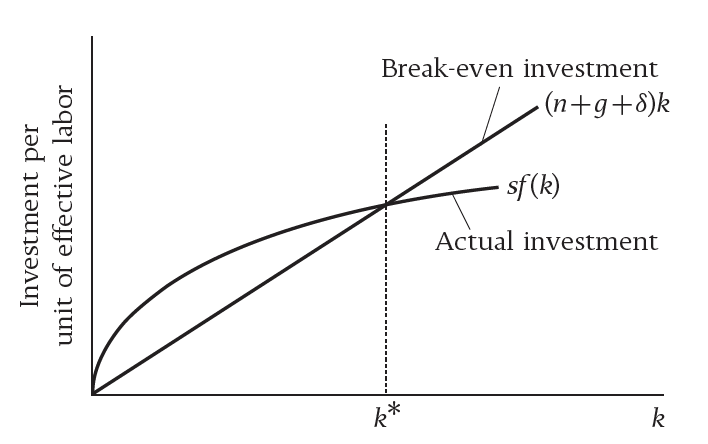
\includegraphics[width=0.6\linewidth]{figures/3_1.png}
				\caption{Dynamic Transition of Capital Per Unit of Effective Labor}
			\end{figure}
			
			\begin{figure}[h]
				\centering
				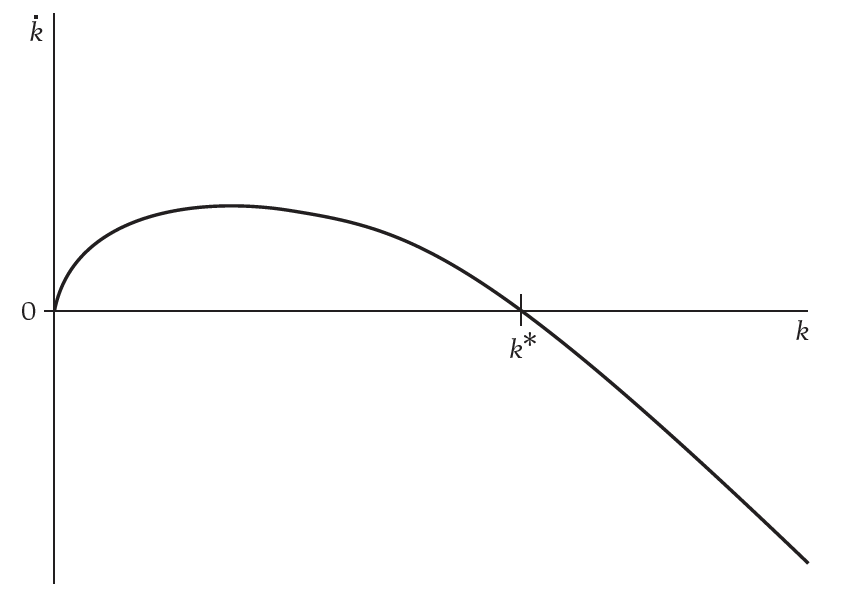
\includegraphics[width=0.6\linewidth]{figures/3_2.png}
				\caption{Phase Diagram of Capital Per Unit of Effective Labor}
			\end{figure}
			
			\newpage 
			
			\begin{definition}
			\textbf{Steady level of capital per unit of effective labor($k^*$)} is defined as the level of capital per unit of effective labor that equates break-even investment per unit of effective labor and actual investment per unit of effective labor. So that $k$ does not deviate from $k^*$.\footnote{The definition can also be expressed as $k^* := \{k \in \R_{+}: \dot{k}(k) = 0\}$}
				\[
					k^* := \{k \in \R_{+}: sf(k) = (n+g+\delta) k\}
				\]
			\end{definition}
			
			\begin{remark}
				The values of other endogenous variables at steady state are derived from $k^*$.
				\begin{example} Find the steady state growth rate of investment, consumption and output per unit of effective labor.
					\begin{gather}
						y^* = f(k^*) \\
						i^* = sf(k^*) = (n+g+\delta) k^* \\
						c^* = y^* - i^* = f(k^*) - (n+g+\delta)k^* = (1-s)f(k^*)
					\end{gather}
				\end{example}
				For the growth rate of each endogenous variable (per unit of effective labor). 
					\begin{gather}
						\pd{i(t)}{t}|_{k=k^*} = 0 \\
						\pd{c(t)}{t}|_{k=k^*} = 0 \\
						\pd{y(t)}{t}|_{k=k^*} = 0 
					\end{gather}
					above relations are equivalent to 
					\begin{gather}
						\tx{On steady state} \begin{cases}
							\dot{i}(t) = 0 \\
							\dot{c}(t) = 0 \\
							\dot{y}(t) = 0 \\
						\end{cases}
					\end{gather}
			\end{remark}
			
			\begin{proof}
				By definition of consumption per unit of effective labor,\\
				$c(\cdot) = (1-s)f(k(t))$ \\
				$\implies \dot{c}(t) := \pd{c(\cdot)}{t} = (1-s)f'(k(t)) \dot{k(t)}$ by chain rule \\
				Since $\dot{k}|_{k=k^*} = 0$ and $(1-s)f'(k(t)) < \infty$ \\
				Thus $\dot{c}(t)|_{k=k^*} = 0$ \\
				And $i(t) = sf(k(t))$, which is constant at $sf(k^*)$ at steady state. \\
			\end{proof}
			
		\subsection{Balanced Growth Path}
			\begin{definition}
				A \textbf{balanced growth path} is a situation where each variable in the model are all growing at a constant rate. \footnote{Variables are not required to grow at the same rate by this definition.} \footnote{Variables remaining fixed are also considered as growing at a constant rate ($g=0$).}
			\end{definition}
			
			\subsubsection{Growth Rates on Balanced Growth Path}
			\paragraph{Population and Technology} By definition of population and technological progress,
			\begin{gather}
				g_A := \frac{\dot{A}}{A} = g \\
				g_L := \frac{\dot{L}}{L} = n
			\end{gather}
			
			\paragraph{Capital per person} Since $\frac{K(t)}{L(t)} = \frac{k(t)A(t)L(t)}{L(t)} = k(t)A(t)$, and the growth rate of $x(t)$ can be found as $\pd{\ln{x(t)}}{t}$. Then
			\begin{proof}[Solution]
				\begin{gather*}
					\pd{\ln{\frac{K(t)}{L(t)}}}{t} = \pd{k(t)A(t)}{t} \\
					= \pd{\ln{k(t)}}{t} + \pd{\ln{A(t)}}{t} \\
					= \frac{\dot{k}(t)}{k(t)} + g \\
				\end{gather*}
				And at the steady state, by definition, $\dot{k}(t)|_{k-k^*} = 0$, therefore 
				\begin{equation}
					\textcolor{blue}{
						g_{\frac{K}{L}}^* = g
					}
				\end{equation}
			\end{proof}
			
			\paragraph{Output and Consumption per person} Similarly,
			\begin{proof}[Solution]
				\begin{gather*}
					\frac{Y(t)}{L(t)} = y(t)A(t) \\
					g_{\frac{Y}{L}} = \pd{\ln{y(t)} + \ln{A(t)}}{t} \\
					= \pd{\ln{y}}{t} + \pd{\ln{A(t)}}{t} \\
					= g + \frac{\dot{y}}{y}
				\end{gather*}
				and for consumption per person,
				\begin{gather*}
					\frac{C(t)}{L(t)} = c(t)A(t)\\
					g_{\frac{C}{L}} = g + \frac{\dot{c}}{c} \\
				\end{gather*}
				Thus, on the balanced growth path, \footnote{$g_X^*$ denotes the growth rate of variable $X$ on the balanced growth path.}
				\begin{gather}
					\textcolor{blue}{
						g_{\frac{Y}{L}}^* = g
					}
					\\
					\textcolor{blue}{
						g_{\frac{C}{L}}^* = g
					}
				\end{gather}
			\end{proof}
			
			\begin{proposition}
				Along the balanced growth path, consumption and output per person also grow at rate $g$.
			\end{proposition}
			
			\begin{proposition}
				Along the balanced growth path, aggregate variables, $Y(t), I(t), C(t)$ are all growing at a rate $n + g$.
				\begin{equation}
					\textcolor{blue}{
						g_{Y}^* = g_{C}^* = g_{I}^* = n + g
						}
				\end{equation}
			\end{proposition}
			\begin{proof}
				\begin{gather*}
				g_{K} = \pd{\ln{K(t)}}{t} \\
				= \pd{\ln{A(t)L(t)k(t)}}{t} \\
				= \pd{\ln{A(t)}}{t} + \pd{\ln{L(t)}}{t} + \pd{\ln{k(t)}}{t} \\
				= g + n + \frac{\dot{k}}{k}
				\end{gather*}
				and at balanced growth path, $\frac{\dot{k}}{k}|_{k=k^*} = 0$, therefore 
				\begin{equation}
					\textcolor{blue}{
						g_K^* = n + g
					}
				\end{equation}
				and proof for $C(t)$ and $I(t)$ follows the same path.
			\end{proof}
		
		\begin{definition}
			The \textbf{golden rule level of capital per unit of effective labor} ($k_G$) is the \ul{steady state level of} capital per unit of effective labor that maximizes steady state consumption per unit of effective labor.
				\[
					k_G = argmax_{k^* \in \textbf{k}^*(\Theta)} \{c^* = f(k^*) - (n+g+ \delta) k^*\}
				\]
		\end{definition}
		
		\begin{definition}
			The \textbf{golden rule level of saving rate} $s_G$ is the saving rate such that the golden role level of capital per unit of effective labor is achieved.
		\end{definition}
		
		\begin{proof}[Proof. (First Order Necessary Condition for $k_G$)]
			\begin{gather*}
				\pd{c^*(k^*)}{k^*} = 0 \\
				\implies \pd{f(k^*) - (n+g+\delta)k^*}{k^*} = 0 \\
				\implies f'(k^*) = (n+g+\delta)
			\end{gather*}
			Thus, golden rule level of capital stock per unit of effective labor $k_G$ can be expressed as \footnote{Notice that the zero solution, $k^* = 0$ is a trivial steady state and we ignore this case during this course.}
			\begin{equation}
				k_G = \{k \in \R_{+}: f'(k) = (n+g+\delta)\}
			\end{equation}
		\end{proof}
		
		\subsection{Experiment}
			\subsubsection{Impact of Change in the Saving Rate ($s_1 > s_0$)}
			\par Suppose at time $t_0$, the saving rate parameter increases discretely: $s_0 \rightarrow s_1$.
			\begin{figure}[H]
				\centering
				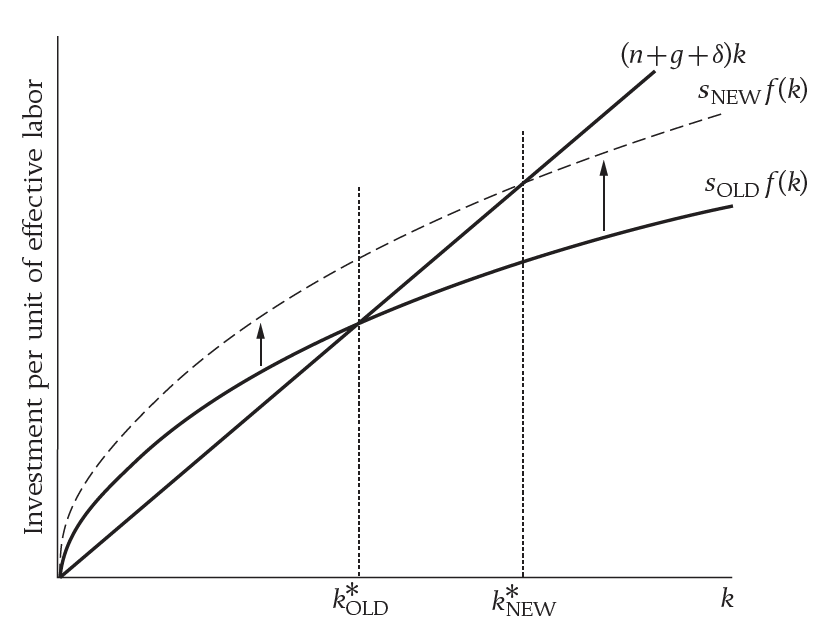
\includegraphics[width=0.5\linewidth]{figures/3_3.png}
				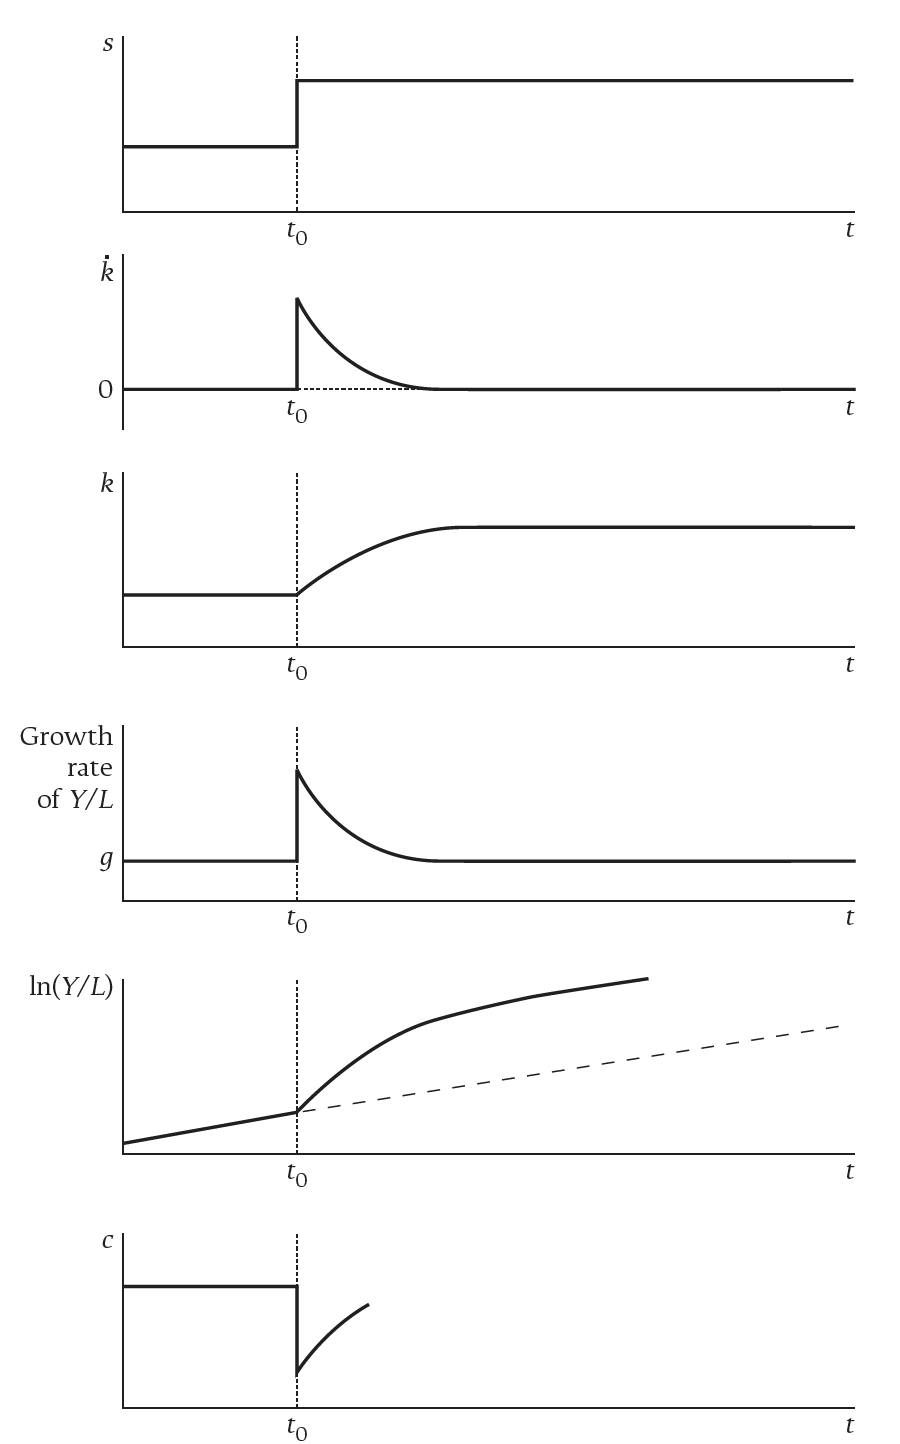
\includegraphics[width=0.5\linewidth]{figures/3_4.png}
				\caption{Effect of an Increase in Saving Rate.}
			\end{figure}
			
			\begin{remark}
				The relation of $c_0^*$ and $c_1^*$ depends on the relative position of $s_1$ and the golden rule level of saving rate $s_G$.
			\end{remark}
			
			\subsubsection{Derive the Effect of Change in $s$ Mathematically}
				\paragraph{Goal} Find $\pd{k^*}{s}$. And notice that $k^*(n+g+\delta) = sf(k^*)$ for any steady state capital level $k^*$. And the steady state level of capital per unit of effective labor can be written as a function of parameters, as $k^*(n, g, \delta, s)$.
				
			\paragraph{Impact on $k^*$}
			\begin{proof}[Solution]
				At any steady state level, $k^*$ satisfies \\
				\[sf(k^*(n,g,\delta,s)) = (n+g+\delta)k^*(n,g,\delta,s)\] \\
				Differentiate both sides with respect to $s$, \\
				We have \[sf'(k^*)\pd{k^*}{s} + f(k^*) = (n+g+\delta)\pd{k^*}{s}\] \\
				Rearrange and get \\
				\[
					\pd{k^*}{s} = \frac{f(k^*)}{(n+g+\delta) - sf'(k^*)}
				\] \\
				Notice that the slope of break-even investment is greater than the slope of the actual investment at the steady state, therefore \[\pd{k^*}{s} > 0\] \\
			\end{proof}
			
			\paragraph{Impact on $y^*$}
			\begin{proof}[Solution]
				Using chain rule we have
				\begin{gather*}
					\pd{y^*}{s} = \pd{f(k^*)}{s} \\
					= \pd{f(k^*)}{k^*} \pd{k^*}{s} > 0,\ \forall k^* \in \textbf{k}^*({\Theta})
				\end{gather*}
			\end{proof}
			
			\par To get a sense on how much $y^*$ changes wit respect to change in $s$, we could look at the \ul{elasticity}.
			\[
				\eta = \pd{y^*}{s}\frac{s}{y^*} = f'(k^*) \pd{k^*}{s} \frac{s}{f(k^*)} = \frac{f'(k^*)s}{(n+g+\delta) - sf'(k^*)}
			\]
			Recall that $(n+g+\delta) = \frac{sf(k^*)}{k^*}$ and rearrange the elasticity
			\begin{gather*}
				\eta = \pd{y^*}{s}\frac{s}{y^*} \\
				= \frac{f'(k^*)s}{(n+g+\delta) - sf'(k^*)} \\
				= \frac{s f'(k^*)}{\frac{s f(k^*)}{k^*} - sf'(k^*)} \\
				= \frac{f'(k^*)}{\frac{f(k^*)}{k^*} - f'(k^*)} \\
				= \frac{f'(k^*) \frac{k^*}{f(k^*)}}{1 - f'(k^*)\frac{k^*}{f(k^*)}} \\
				= \textcolor{blue}{
					\frac{\alpha_K}{1 - \alpha_K}
					} \\
			\end{gather*}
			
			\begin{remark}
				$\alpha_K$ denotes the elasticity of output per unit of effective unit labor with respect to capital stock per unit of effective labor, along the balanced growth path. And
				\[
					\alpha_K \approx \frac{1}{3}
				\]
			\end{remark}
			
			\begin{remark}
				If the production function is in the Cobb-Douglas form, then $\alpha_K = \alpha$.
			\end{remark}
			
			\begin{example}
				If $\alpha_K \approx \frac{1}{3}$ then \[\eta = \pd{y^*}{s} \frac{s}{y^*} \approx \frac{1}{2}\]
			\end{example}
			
			\paragraph{Impact on $c^*$} Notice that on the balanced growth path $c^* = y^* - i^*$.
			\begin{equation}
				c^* = f(k^*) - (n+g+\delta)k^*
			\end{equation}
			and differentiate with respect to $s$
			\[
				\pd{c^*}{s} = [f'(k^*) - (n+g+\delta)] \pd{k^*}{s}
			\]
			And notice that the sign of $\pd{c^*}{s}$ depends on the relative slope of production function and break-even investment.
			By the first order condition of golden rule level of capital per unit of effective labor, $(n+g+\delta) = f'(k_G)$
			\begin{gather*}
				\pd{c^*}{s} = [f'(k^*) - f'(k_G)]\pd{k^*}{s}
			\end{gather*}
			And 
			\begin{equation*}
				\begin{cases}
					k^* = k_G \implies f'(k^*) = f'(k_G) \implies \pd{c^*}{s} = 0 \\
					k^* < k_G \implies f'(k^*) > f'(k_G) \implies \pd{c^*}{s} > 0 \\
					k^* > k_G \implies f'(k^*) < f'(k_G) \implies \pd{c^*}{s} < 0
				\end{cases}
			\end{equation*}
	\section{Lecture 4 September 27. 2018}
	\subsection{Speed of Convergence}
	    \paragraph{Methodology} Look at the change in $k$ and linearize using first order Taylor's expansion.
	    \paragraph{Recall} $\dot{k}(t)$ is a function of $k(t)$ since 
	    \begin{equation}
	        \dot{k}(t) = sf(k(t)) - (n+g+\delta)k(t)
	    \end{equation}
	    And the first order Taylor series approximation of a function $f(x)$ around the point $x = x_0$.
	    \[
	        f(x) \approx f(x_0) + f'(x_0)(x - x_0)
	    \]
	    Then
	    \begin{gather*}
	        \dot{k}(k) \approx \dot{k}(k^*) + \pd{\dot{k}(k)}{k}|_{k=k^*} (k - k^*) \\
	        = 0 + \pd{\dot{k}(k)}{k}|_{k=k^*} (k - k^*)
	    \end{gather*}
	    Differentiating the both sides of equation (1) with respect to $k$.
	    \begin{gather*}
	        \pd{\dot{k}(k)}{k}|_{k=k^*} = sf'(k^*) - (n + g + \delta) \\
	        = \frac{(n + g + \delta) k^*}{f(k^*)} f'(k^*) - (n + g + \delta) \\
	        = (n + g + \delta) \Big [
	            \frac{f'(k^*) k^*}{f(k^*)} - 1
	            \Big ] \\
	        = (n + g + \delta) (\alpha (k^*) - 1)
	    \end{gather*}
	    where 
	    \begin{equation}
	    \textcolor{blue}{
	        \alpha_k (k^*) = f'(k^*)\frac{k^*}{f(k^*)}
	        }
	    \end{equation}
	    denotes the \ul{elasticity of $y$ with respect to $k$ \emph{at steady state}.}
	    So
	    \begin{gather*}
	        \dot{k}(k(t)) \approx (n + g + \delta) (\alpha (k^*) - 1) (k(t) - k^*) \\
	        \implies \pd{({k - k^*}(k))}{t} = \dot{k}(k(t)) \approx (n + g + \delta) (\alpha (k^*) - 1) (k(t) - k^*)
	    \end{gather*}
	    Let $\lambda := (n + g + \delta) (1 - \alpha (k^*))$ then 
	    \begin{gather}
	    \textcolor{orange}{
	        k(t) - k^* \approx e^{-\lambda t}(k(0) - k^*)
	    }
	    \end{gather}
	    \begin{remark}
		    \begin{proof}[Derive] (above equation)\\
		        Let $X(t) := k(t) - k^*$ \\
		        And since $\pd{k(t)}{t} = \pd{(k(t) - k^*)}{t}$ \\
		        Therefore $\dot{X}(t) = \dot{k}(t) \approx -\lambda X(t)$ \\
		        $\implies X(t) \approx X(0) e^{-\lambda t}$ \\
		        $\iff k(t) - k^* \approx (k(0) - k^*) e^{-\lambda t}$
		    \end{proof}
	    \end{remark}
	    Then note that 3
	    \begin{gather*}
	        y(t) = f(k(t)) \\
	        \implies \dot{y}(t) = f'(k(t))\dot{k}(t) \\
	        \tx{(Take the first order Taylor series approximation around $k=k^*$)} \\
	        \implies y(t) \approx f(k^*) + f'(k^*) (k(t)-k^*) \\
	        \implies y(t) - y^* \approx f'(k^*)(k(t) - k^*) \\
	        \implies \frac{\dot{y}(t)}{y(t) - y^*} = \frac{f'(k^*)\dot{k}(t)}{f'(k^*)(k(t) - k^*)} = \frac{\dot{k}(t)}{k(t) - k^*} \approx - \lambda \\
	       \implies \textcolor{orange}{
	       		y(t) - y^* \approx e^{- \lambda t} (y(0) - y^*)
	       }
	    \end{gather*}
	    
	    \begin{example}
	        How long does it take to move 1/2 way to the balance growth path. Assuming population growth rate is $2\%$, growth in output per worker is $2\%$ and depreciation is $2\%$ and  $\alpha_K = \frac{1}{3}$.
	        \begin{proof}[Solution]
	            $\lambda = (1 - \alpha_K)(n + g + \delta)$ 
	            Since we know along the balanced growth path, \begin{gather*}
	                \frac{Y(t)}{L(t)} = y^* A(t) \\
	                \implies \pd{\ln{\frac{Y(t)}{L(t)}}}{t} = g
	            \end{gather*}
	            Therefore $g = 0.02$ and therefore $\lambda = 0.04$. \\
	            To find the date where we have moved half way we need to solve 
	            \begin{gather*}
	                \frac{y(\tilde{t}) - y^*}{y(0) - y^*} = 0.5 \approx e^{-\lambda t}\\
	                \implies \ln(0.5) \approx -\lambda \tilde{t} \\
	                \implies \tilde{t} = \frac{-\ln(0.5)}{0.04} \approx 17.33
	            \end{gather*}
	        \end{proof}
	    \end{example}
	    
	    \subsection{General Statements}
	    \par Solow growth model identifies 2 sources of output \ul{per worker},
	    \begin{enumerate}
	    	\item Differences in the among of \ul{capital per worker}.
	    	\item Differences in the \ul{effectiveness of productivity} of labor $A$.
	    \end{enumerate}
	    Notice that the output per worker 
	    \[
	    	\frac{Y(t)}{L(t)} = \frac{F(K(t), A(t)L(t))}{L(t)} = F(\frac{K(t)}{L(t)}, A(t))
	    \]
	    Notice that in the long run balanced growth path
	    \begin{gather*}
	    	\frac{K(t)}{L(t)} = k(t)A(t) \\
	    	\implies \pd{\ln(\frac{K(t)}{L(t)})}{t} = \frac{\dot{k}(t)}{k(t)} + \frac{\dot{A}(t)}{A(t)}
	    \end{gather*}
	    Therefore along the balanced growth path $\dot{k}(t) = 0$ so only the growth in $A$ matters.
	    
	    \subsection{Growth Accounting}
	    \par Consider the growth rate of aggregate output $Y(t)$, take the total differential and get
	    \begin{gather}
	    	\dot{Y}(t) = \pd{Y(t)}{K(t)} \pd{K(t)}{t} + \pd{Y(t)}{L(t)} \pd{L(t)}{t} + \pd{Y(t)}{A(t	)}\pd{A(t)}{t} \\
	    	\implies 
	    	\frac{\dot{Y}(t)}{Y(t)} = \pd{Y(t)}{K(t)} \frac{1}{Y(t)} \pd{K(t)}{t} + \pd{Y(t)}{L(t)} \frac{1}{Y(t)} \pd{L(t)}{t} + \pd{Y(t)}{A(t)} \frac{1}{Y(t)} \pd{A(t)}{t} 
	    \end{gather}
	    Then express the equation in terms of growth rates in $K, L, A$ variables,
	    \begin{gather}
	    	\frac{\dot{Y}(t)}{Y(t)} = \textcolor{orange}{\pd{Y(t)}{K(t)} \frac{K(t)}{Y(t)}}\frac{\pd{K(t)}{t}}{K(t)} 
	    	+ \textcolor{red}{\pd{Y(t)}{L(t)} \frac{L(t)}{Y(t)}} \frac{\pd{L(t)}{t}}{L(t)} 
	    	+ \textcolor{blue}{\pd{Y(t)}{A(t)} \frac{A(t)}{Y(t)} \frac{\pd{A(t)}{t}}{A(t)}}
	    	\\
	    	= \textcolor{orange}{\alpha_K} \frac{\dot{K}(t)}{K(t)} 
	    	+ \textcolor{red}{\alpha_L} \frac{\dot{L}(t)}{L(t)} 
	    	+ \textcolor{blue}{R(t)}
	    \end{gather}
	    where $R(t)$ is the \textbf{Solow Residual} and 
	    \begin{equation}
	    	\textcolor{blue}{R(t) = \pd{Y(t)}{A(t)} \frac{A(t)}{Y(t)} \frac{\dot{A}(t)}{A(t)}}
	    \end{equation}
	    And $\alpha_K(t)$ and $\alpha_L(t)$ denote the elasticity of output with respect to capital and labor respectively.
	    
	    \begin{example}
	    	Assume the output growth is $40\%$ and capital growth is $20\%$ and labor growth is $30\%$. If $\alpha_K = 0.3$ and $\alpha_L = 0.7$. What's the contribution to output growth of capital?
	    	\[
	    		\alpha_K \frac{\dot{K}(t)}{K(t)} = 0.3 \times 20\% = 0.06
	    	\]
	    	and the contribution from labor is
	    	\[
	    		\alpha_L \frac{\dot{L}(t)}{L(t)} = 0.7 \times 30\% = 0.21
	    	\]
	    	and the Solow residual is 
	    	\[
	    		R(t) = g_Y - 6\% - 21\% = 0.4 - 0.06 - 0.21 = 0.13
	    	\]
	    \end{example}
	    
	    \begin{example}
	    	Let's assume the economy is on its balanced growth path. Assume that a change in medicine increase survival rate during child birth. \\
	    	What would the effect of this be on steady state $k^*, y^*, c^*, i^*$.\\
	    	First show the growth that despite break-even investment and actual investment. Label the steady state values. \\
	    \end{example}
	    
	    \begin{proof}[Solution]
	    	\textbf{The effect would be an increase in $n$} \\
	    	Suppose $n_0 \to n_1$ with $n_0 < n_1$. \\
	    	Therefore $k^*$ falls, and $y^*$ falls. \\
	    	Since consumption and actual investment are constant frictions of $y^*$, \\
	    	Therefore both $c^*, i^*$ falls.
	    	\begin{figure*}[h]
	    		\centering
	    		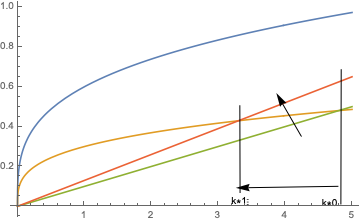
\includegraphics[width=0.7\linewidth]{figures/4_1}
	    	\end{figure*}
	    \end{proof}
	
	\section{Lecture 5}
	\subsection{Economy}
	\begin{itemize}
		\item Infinite horizon continuous time model.
		\item Exogenous growth rates of technology and population.
		\begin{gather*}
			A(t) = A(0) e^{gt} \\
			L(t) = L(0) e^{nt}
		\end{gather*}
		\item A key difference from the solow model is that the saving decision and the capital stock are determined by the interaction of maximizing households and firms.
	\end{itemize}
	
	\subsection{Households}
	\begin{assumption}(Household Setup)
		\begin{itemize}
			\item There are a large numbers of \ul{identical} households in the economy ($H$). \emph{To ensure that \ul{no household has marker power}.}
			\item And the size of each household are assumed to grow at rate $n$.
			\item Each household has $\frac{L(t)}{H}$ people in it at time $t$.
			\item Each household has initial capital holding of $\frac{K(0)}{H}$.
			\item Each member of the household supplies 1 unit of labor at each point in time \ul{inelastically}. (\emph{No uncertainty})
			\item (For simplicity)There's no depreciation. ($\delta = 0$)
			\item Capital is rented to firms at rate $r(t)$.
			\item Labor is hired at rate $W(t) = w(t)A(t)$. Where $W(t)$ is the wage per unit of labor and $w(t)$ is the wage per unit of effective labor.
		\end{itemize}
	\end{assumption}
	
	\paragraph{Objective Function} Household's \textbf{lifetime utility function} is given by
	\begin{equation}
		\textcolor{orange}{
			U = \int_{t=0}^\infty {e^{-\rho t} u(C(t)) \frac{L(t)}{H}}\ dt
		}
	\end{equation}
	where $\rho$ is the \textbf{discount rate} and $C(t)$ is the \textbf{consumption per person}.
	\begin{remark}
		When $\rho = 0$, household values utility in the future equally. The greater $\rho$ is, the less value household puts on future consumption/utility.
	\end{remark}
	
	\paragraph{Household Budget Constraints} Household's budget is given in terms of \ul{present discounted value}. \\
	Since the household has $\frac{L(t)}{H}$ members, labor income at time $t$ is 
	\[
		A(t)w(t)\frac{L(t)}{H} = W(t)\frac{L(t)}{H}
	\]
	\\
	The amount of consumption for the household at the time $t$ is 
	\[
		C(t)\frac{L(t)}{H}
	\]
	And let $R(t)$ denote the \textbf{continuous compounding interest rate}:
	\begin{equation}
		R(t) := \int_{\tau=0}^t r(\tau)\ d\tau
	\end{equation}
	\begin{remark}
		We know under \ul{continuously compounding interest}, one unit of output invested at time 0 is worth $e^{R(t)}$ units at time $t$. Conversely, 1 unit of output at time $t$ is worth $e^{-R(t)}$ at time 0.
	\end{remark}
	\begin{remark}
		The budget constraint implies that the \ul{present discounted value of lifetime consumption} cannot exceed the \ul{present discounted value of labor income} plus \ul{initial wealth}.
	\end{remark}
	\par And the household lifetime budget constraint is given by
	\begin{equation}
		\textcolor{orange}{
			\int_{t=0}^\infty e^{-R(t)} C(t) \frac{L(t)}{H}\ dt \leq \frac{K(0)}{H} + \int_{t=0}^\infty e^{-R(t)} w(t) \frac{A(t)L(t)}{H}\ dt
		}
	\end{equation}
	\par Normalize budget constraint (3) into per unit of effective labor variables to get an equivalent form.
	\begin{gather*}
		\int_{t=0}^\infty e^{-R(t)} C(t) \frac{L(t)}{H}\ dt  \leq \frac{K(0)}{H} + \int_{t=0}^\infty e^{-R(t)} w(t) \frac{A(t)L(t)}{H}\ dt \\
		\iff 
		\int_{t=0}^\infty e^{-R(t)} c(t) \frac{A(t)L(t)}{H}\ dt \leq \frac{k(0)A(0)L(0)}{H} + \int_{t=0}^\infty e^{-R(t)} w(t) \frac{A(t)L(t)}{H}\ dt \\ 
		\iff \int_{t=0}^\infty e^{-R(t)} c(t) e^{(n+g)t} \frac{A(0)L(0)}{H}\ dt \leq \frac{k(0)A(0)L(0)}{H} + \int_{t=0}^\infty e^{-R(t)} w(t) e^{(n+g)t}\frac{A(0)L(0)}{H}\ dt \\
		\iff \int_{t=0}^\infty e^{-R(t)} e^{(n+g)t} c(t)\ dt \leq k(0) + \int_{t=0}^\infty e^{-R(t)} e^{(n+g)t} w(t)\ dt
	\end{gather*}
	\par About \textbf{assets} on date $t=s$, notice
	\begin{gather*}
		\frac{K(s)}{H} = \frac{K(0)}{H}e^{R(s)} + \int_{t=0}^s e^{-R(t)+R(s)} \Big\{\frac{w(t)A(t)L(t)}{H} - \frac{c(t)A(t)L(t)}{H} \Big\}\ dt \\
		= \frac{K(0)}{H} e^{R(s)} +  \int_{t=0}^s e^{-R(t)+R(s)} \{w(t) - c(t)\} \frac{A(t)L(t)}{H} dt \\
		\implies \frac{K(s)}{H}e^{-R(s)} := \frac{K(0)}{H} + \int_{t=0}^s e^{R(t)} \{w(t) - c(t)\} \frac{A(t)L(t)}{H}\ dt
	\end{gather*}
	Back to the budget constraint,
	\begin{gather*}
		\frac{K(0)}{H} + \int_{t=0}^\infty \frac{w(t)A(t)L(t)}{H}\ dt - \int_{t=0}^\infty \frac{c(t)A(t)L(t)}{H}\ \geq 0 \\
		\iff \frac{K(0)}{H} + \int_{t=0}^\infty e^{-R(t)} \{w(t) - c(t)\} \frac{A(t)L(t)}{H} \geq 0 \\
		\iff \lim_{s \to \infty}\Big\{ \frac{K(0)}{H} + \int_{t=0}^s e^{-R(t)} \{w(t) - c(t)\} \frac{A(t)L(t)}{H} \geq 0 \Big \} \\
		\implies \lim_{s\to \infty}e^{-R(s)}\frac{K(s)}{H} \geq 0
	\end{gather*}
	These implies that the household's asset holding cannot be negative in the limit. And this is a \textbf{no-Ponzi game} condition.
	
	\begin{definition}
		A \textbf{Ponzi-game} is a scheme in which someone issues debt and rolls it over forever. In other words, the person always pays off debt by issuing more debt.
	\end{definition}
	
	\begin{remark}
		If households could run a Ponzi scheme, then the present value of lifetime consumption can exceed the present value of lifetime resources.
	\end{remark}
	The household instantaneous utility function (CRRA).
	\begin{equation}
		u(C(t)) = \frac{C(t)^{1 - \theta}}{1 - \theta}
	\end{equation}
	\begin{assumption}
		Assuming $\theta > 0$ and $\beta = \rho - n - (1-\theta)g > 0$.
	\end{assumption}
	\begin{gather*}
		U = \int_{t=0}^\infty e^{-\rho t} \frac{c(t)^{1-\theta}}{1-\theta} A(0)^{1-\theta} e^{(1-\theta)gt} e^{nt} \frac{L(0)}{H}\ dt\\
		= A(0)^{1 - \theta} \frac{L(0)}{H} \int_{t=0}^\infty {e^{-\rho t + nt + (1-\theta)gt} \frac{c(t)^{1-\theta}}{1-\theta}\ dt} \\
		= A(0)^{1 - \theta} L(0) \int_{t=0}^\infty {e^{-(\rho - n - (1-\theta)g)t} \frac{c(t)^{1-\theta}}{1-\theta}\ dt} \\
		= B \int_{t=0}^\infty e^{-\beta t}\frac{c(t)^{1-\theta}}{1- \theta}\ dt \\
	\end{gather*}
	\begin{remark}
		If $\beta \leq 0$ then the integral would diverge and the maximization problem does not have a well-defined solution.
	\end{remark}
\end{document}




























